\section{Additional results}

We present full results of materials from the main paper as well as  additional results in Figures~\ref{fig:results-a}--\ref{fig:results-c}. The presentation follows the main paper and shows results of our complete pipeline starting from basic assets all the way to the recovered material parameters.

Figure~\ref{fig:attention_viz_suppl} shows an uncropped version of Figure~\ref{fig:attention_viz} in the main paper, and visualizes exemplary attention scores before and after adding the bias for a single specific
surface point.

Finally, Figure~\ref{fig:hparams_usercontrol_suppl} is an extended version of Figure~\ref{fig:hparams_usercontrol} from the main paper and demonstrates the full set of user-controlled parameters and their impact on the generated visuals. The \emph{classifier-free guidance} parameter controls the amount of adherence to the prompt; the \emph{CNet Tile scale} and the added noise parameters control how much the generated material is allowed to deviate from the input views, and trades off the amount of detail vs preservation of the original design intent.

\newcommand{\supplpadthree}[1]{%
  \ifnum#1<10 00#1\else%
  \ifnum#1<100 0#1\else%
  #1%
  \fi\fi%
}

\newcommand{\supplnewsceneblock}[6]{%
\begin{tabular}{cccccc}
    \multicolumn{6}{>{\centering\arraybackslash}p{\textwidth}}{#2} \\
    \multicolumn{2}{c}{(a) Conditioning renders} &
    \multicolumn{2}{c}{(b) Diffusion outputs} &
    \multicolumn{2}{c}{(c) Reconstructed material} \\
    \begin{overpic}[width=0.16\textwidth]{figures/results/#1/initial_rendering_\supplpadthree{#3}.jpg}
        \put(2,2){\tiny\textcolor{white}{View #3}}
    \end{overpic}
    &
    \begin{overpic}[width=0.16\textwidth]{figures/results/#1/initial_rendering_\supplpadthree{#4}.jpg}
        \put(2,2){\tiny\textcolor{white}{View #4}}
    \end{overpic}
    &
    \begin{overpic}[width=0.16\textwidth]{figures/results/#1/diffused_\supplpadthree{#3}.jpg}
        \put(2,2){\tiny\textcolor{white}{View #3}}
    \end{overpic}
    &
    \begin{overpic}[width=0.16\textwidth]{figures/results/#1/diffused_\supplpadthree{#4}.jpg}
        \put(2,2){\tiny\textcolor{white}{View #4}}
    \end{overpic}
    &
    \begin{overpic}[width=0.16\textwidth]{figures/results/#1/masked/recovered_default_\supplpadthree{#3}.jpg}
        \put(2,2){\tiny\textcolor{white}{View #3}}
    \end{overpic}
    &
    \begin{overpic}[width=0.16\textwidth]{figures/results/#1/masked/recovered_default_\supplpadthree{#4}.jpg}
        \put(2,2){\tiny\textcolor{white}{View #4}}
    \end{overpic}
    \\
    \begin{overpic}[width=0.16\textwidth]{figures/results/#1/initial_rendering_\supplpadthree{#5}.jpg}
        \put(2,2){\tiny\textcolor{white}{View 4}}
    \end{overpic}
    &
    \begin{overpic}[width=0.16\textwidth]{figures/results/#1/initial_rendering_\supplpadthree{#6}.jpg}
        \put(2,2){\tiny\textcolor{white}{View #6}}
    \end{overpic}
    &
    \begin{overpic}[width=0.16\textwidth]{figures/results/#1/diffused_\supplpadthree{#5}.jpg}
        \put(2,2){\tiny\textcolor{white}{View #5}}
    \end{overpic}
    &
    \begin{overpic}[width=0.16\textwidth]{figures/results/#1/diffused_\supplpadthree{#6}.jpg}
        \put(2,2){\tiny\textcolor{white}{View #6}}
    \end{overpic}
    &
    \begin{overpic}[width=0.16\textwidth]{figures/results/#1/masked/recovered_default_\supplpadthree{#5}.jpg}
        \put(2,2){\tiny\textcolor{white}{View #5}}
    \end{overpic}
    &
    \begin{overpic}[width=0.16\textwidth]{figures/results/#1/masked/recovered_default_\supplpadthree{#6}.jpg}
        \put(2,2){\tiny\textcolor{white}{View #6}}
    \end{overpic}
    \\
    \midrule
    (d) Initial albedo & (e) Reconstructed albedo & (f) Initial normal & (g) Reconstructed normal & (h) Initial roughness & (i) Reconstructed roughness \\
    \includegraphics[width=0.16\textwidth]{figures/results/#1/texture_albedo_initial.jpg} &
    \includegraphics[width=0.16\textwidth]{figures/results/#1/texture_albedo_edited.jpg} &
    \includegraphics[width=0.16\textwidth]{figures/results/#1/texture_normals_initial.jpg} &
    \includegraphics[width=0.16\textwidth]{figures/results/#1/texture_normals_edited.jpg} &
    \includegraphics[width=0.16\textwidth]{figures/results/#1/texture_roughness_initial.jpg} &
    \includegraphics[width=0.16\textwidth]{figures/results/#1/texture_roughness_edited.jpg}
    \vspace*{4mm}
\end{tabular}
}

\begin{figure*}
    \centering%
    \setlength{\tabcolsep}{0.002\textwidth}%
    \renewcommand{\arraystretch}{1}%
    \footnotesize%
    \supplnewsceneblock{briefcase}{\small Briefcase, prompt: \prompt{Old, overused, weathered, scratched, leather briefcase}}{0}{1}{4}{5}
    \supplnewsceneblock{david}{\small David bust, prompt \prompt{Old, cracked statue of David}}{0}{1}{4}{5}
    \vspace*{-6mm}
    \caption{We use renderings of the original asset (two pairs of two adjacent views are shown in (a)) to condition the diffusion model to produce images with enhanced appearance (b), which is then back-propagated into the original material definition. In (c), we show the resulting asset on four frames from a turntable animation (we picked frames that correspond to the conditioning views); see the accompanying video for the full animation.
    Columns (d) to (i) show albedo, normal, and roughness textures of the initial and reconstructed material.
    }
    \label{fig:results-a}
\end{figure*}


\begin{figure*}
    \centering%
    \setlength{\tabcolsep}{0.002\textwidth}%
    \renewcommand{\arraystretch}{1}%
    \footnotesize%
    \supplnewsceneblock{pots}{\small Pottery Vases, prompt: \prompt{Weathered pottery vases}}{0}{2}{10}{12}
    \supplnewsceneblock{pot-simple}{\small Cooking Pot, prompt \prompt{rusty scratched old cooking pot}}{0}{1}{7}{8}
    \vspace*{-6mm}
    \caption{We use renderings of the original asset (two pairs of two adjacent views are shown in (a)) to condition the diffusion model to produce images with enhanced appearance (b), which is then back-propagated into the original material definition. In (c), we show the resulting asset on four frames from a turntable animation (we picked frames that correspond to the conditioning views); see the accompanying video for the full animation.
    Columns (d) to (i) show albedo, normal, and roughness textures of the initial and reconstructed material.
    }
    \label{fig:results-b}
\end{figure*}


\begin{figure*}
    \centering%
    \setlength{\tabcolsep}{0.002\textwidth}%
    \renewcommand{\arraystretch}{1}%
    \footnotesize%
    \supplnewsceneblock{woodenbox}{\small Wooden Box, prompt: \prompt{Aged, old, weathered wooden box}}{1}{2}{14}{15}
    \supplnewsceneblock{greekvase}{\small Greek Vase, prompt \prompt{A highly detailed ancient Greek vase, decorated with intricate mythological patterns and scenes of warriors, partially cracked and chipped from age, with areas of fading paint and earthy dust coating its surface. The vase is surrounded by a soft warm light. The style is realistic and cinematic, emphasizing texture and detail, with a focus on the cracks and aged patina on the vase.}}{4}{5}{10}{11}
    \vspace*{-6mm}
    \caption{We use renderings of the original asset (two pairs of two adjacent views are shown in (a)) to condition the diffusion model to produce images with enhanced appearance (b), which is then back-propagated into the original material definition. In (c), we show the resulting asset on four frames from a turntable animation (we picked frames that correspond to the conditioning views); see the accompanying video for the full animation.
    Columns (d) to (i) show albedo, normal, and roughness textures of the initial and reconstructed material.
    }
    \label{fig:results-c}
\end{figure*}

\begin{figure*}[h!]
    \centering%
    \setlength{\tabcolsep}{0.002\textwidth}%
    \renewcommand{\arraystretch}{1}%
    \footnotesize%
    \begin{tabular}{ccc}
        Unmodified attention scores
        &
        Latent pixel correspondences
        &
        Biased attention scores
        \\[0.8mm]
        \begin{overpic}[width=0.332\textwidth]{figures/attnviz/correspondences.jpg}
            \begin{tikzpicture}[overlay, remember picture]
                \draw[-{Stealth[length=2mm]},green,thick,] (3.50,5.20) -- (3.12,4.73);
                \draw[-{Stealth[length=2mm]},red,thick,]   (1.45,5.25) -- (1.07,4.78);
                \draw[-{Stealth[length=2mm]},red,thick,]   (5.63,5.25) -- (5.25,4.78);
                \draw[-{Stealth[length=2mm]},red,thick,]   (4.27,1.31) -- (4.65,0.84);
                \draw[-{Stealth[length=2mm]},red,thick,]   (2.30,1.26) -- (2.68,0.79);
            \end{tikzpicture}
        \end{overpic}
        &
        \begin{overpic}[width=0.332\textwidth]{figures/attnviz/unbiased.jpg}
        \end{overpic}
        &
        \begin{overpic}[width=0.332\textwidth]{figures/attnviz/biased.jpg}
            \begin{tikzpicture}[overlay, remember picture]
                \draw[-{Stealth[length=2mm]},red,thick,]   (1.45,5.25) -- (1.07,4.78);
                \draw[-{Stealth[length=2mm]},red,thick,]   (5.63,5.25) -- (5.25,4.78);
                \draw[-{Stealth[length=2mm]},red,thick,]   (4.27,1.31) -- (4.65,0.84);
                \draw[-{Stealth[length=2mm]},red,thick,]   (2.30,1.26) -- (2.68,0.79);
            \end{tikzpicture}
        \end{overpic}
    \end{tabular}
    \caption{
        An uncropped version of Figure~\ref{fig:attention_viz} from the main paper.
        Left:
        For one latent pixel (green), we highlight the corresponding neighborhoods in the other conditioning views in red; we use ray tracing to check for occlusions.
        Middle:
        One attention score matrix \emph{row} related to that green latent pixel can be rearranged into an image showing how much it attends to all other latent pixels in one stage of the diffusion model.
        Right:
        We bias the matrix entries in \emph{columns} that correspond to the identified red regions to promote attention---and hence consistency---between these latents.
    }
    \label{fig:attention_viz_suppl}
\end{figure*}


\begin{figure*}[htbp]
    \centering%
    \setlength{\tabcolsep}{0.002\textwidth}%
    \renewcommand{\arraystretch}{1}%
    \footnotesize%

    \begin{tabular}{cccccccc}
        &Initial asset& \multicolumn{6}{c}{
            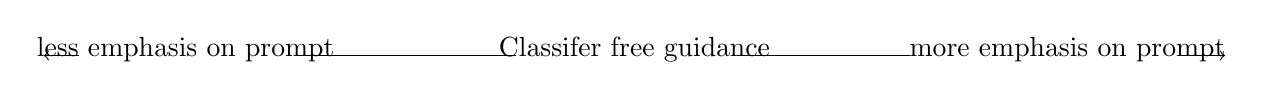
\begin{tikzpicture}
                \draw[<-] (0,0) -- (0.45,0);
                \draw[-] (3.2,0) -- (6.0,0);
                \draw[-] (8.8,0) -- (11,0);
                \draw[->] (14.4,0) -- (15,0);
                \node[above] at (1.8,-0.2) {less emphasis on prompt};
                \node[above] at (7.5,-0.2) {Classifer free guidance};
                \node[above] at (13,-0.2) {more emphasis on prompt};
            \end{tikzpicture}
        }\\[-4pt]%
        && 4.0 & \textbf{7.5} & 11.0 & 14.5 & 18.0 & 21.5\\%
        \rotatebox{90}{\hspace*{4em}View 1}&%
        \includegraphics[height=0.14\linewidth]{figures/secondary_hparams/initial/0001.png}&%
        \includegraphics[height=0.14\linewidth]{figures/secondary_hparams/guidance_4.0_001.jpg}&%
        \includegraphics[height=0.14\linewidth]{figures/secondary_hparams/guidance_7.5_001.jpg}&%
        \includegraphics[height=0.14\linewidth]{figures/secondary_hparams/guidance_11.0_001.jpg}&%
        \includegraphics[height=0.14\linewidth]{figures/secondary_hparams/guidance_14.5_001.jpg}&%
        \includegraphics[height=0.14\linewidth]{figures/secondary_hparams/guidance_18.0_001.jpg}&%
        \includegraphics[height=0.14\linewidth]{figures/secondary_hparams/guidance_21.5_001.jpg}\\%
        \rotatebox{90}{\hspace*{4em}View 2}&
        \includegraphics[height=0.14\linewidth]{figures/secondary_hparams/initial/0006.png}&%
        \includegraphics[height=0.14\linewidth]{figures/secondary_hparams/guidance_4.0_006.jpg}&%
        \includegraphics[height=0.14\linewidth]{figures/secondary_hparams/guidance_7.5_006.jpg}&%
        \includegraphics[height=0.14\linewidth]{figures/secondary_hparams/guidance_11.0_006.jpg}&%
        \includegraphics[height=0.14\linewidth]{figures/secondary_hparams/guidance_14.5_006.jpg}&%
        \includegraphics[height=0.14\linewidth]{figures/secondary_hparams/guidance_18.0_006.jpg}&%
        \includegraphics[height=0.14\linewidth]{figures/secondary_hparams/guidance_21.5_006.jpg}\\%
    \end{tabular}%

    \begin{tabular}{cccccccc}
        &Initial asset& \multicolumn{6}{c}{
            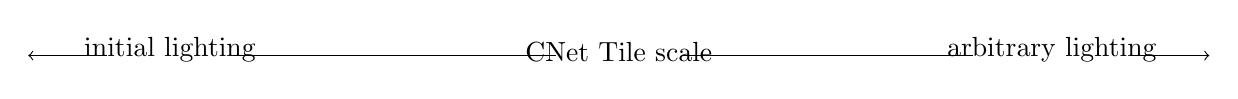
\begin{tikzpicture}
                \draw[<-] (0,0) -- (1,0);
                \draw[-] (2.6,0) -- (6.7,0);
                \draw[-] (8.3,0) -- (12,0);
                \draw[->] (14,0) -- (15,0);
                \node[above] at (1.8,-0.2) {initial lighting};
                \node[above] at (7.5,-0.2) {CNet Tile scale};
                \node[above] at (13,-0.2) {arbitrary lighting};
            \end{tikzpicture}
        }\\[-4pt]%
        && \textbf{1.0} & \textbf{0.8} & 0.6 & 0.4 & 0.2 & 0.0\\%
        \rotatebox{90}{\hspace*{4em}View 1}&%
        \includegraphics[height=0.14\linewidth]{figures/secondary_hparams/initial/0001.png}&%
        \includegraphics[height=0.14\linewidth]{figures/secondary_hparams/tilescale_1.0_001.jpg}&%
        \includegraphics[height=0.14\linewidth]{figures/secondary_hparams/tilescale_0.8_001.jpg}&%
        \includegraphics[height=0.14\linewidth]{figures/secondary_hparams/tilescale_0.6_001.jpg}&%
        \includegraphics[height=0.14\linewidth]{figures/secondary_hparams/tilescale_0.4_001.jpg}&%
        \includegraphics[height=0.14\linewidth]{figures/secondary_hparams/tilescale_0.2_001.jpg}&%
        \includegraphics[height=0.14\linewidth]{figures/secondary_hparams/tilescale_0.0_001.jpg}\\%
        \rotatebox{90}{\hspace*{4em}View 2}&
        \includegraphics[height=0.14\linewidth]{figures/secondary_hparams/initial/0006.png}&%
        \includegraphics[height=0.14\linewidth]{figures/secondary_hparams/tilescale_1.0_006.jpg}&%
        \includegraphics[height=0.14\linewidth]{figures/secondary_hparams/tilescale_0.8_006.jpg}&%
        \includegraphics[height=0.14\linewidth]{figures/secondary_hparams/tilescale_0.6_006.jpg}&%
        \includegraphics[height=0.14\linewidth]{figures/secondary_hparams/tilescale_0.4_006.jpg}&%
        \includegraphics[height=0.14\linewidth]{figures/secondary_hparams/tilescale_0.2_006.jpg}&%
        \includegraphics[height=0.14\linewidth]{figures/secondary_hparams/tilescale_0.0_006.jpg}\\%
    \end{tabular}%

    \begin{tabular}{cccccccc}
        &Initial asset& \multicolumn{6}{c}{
            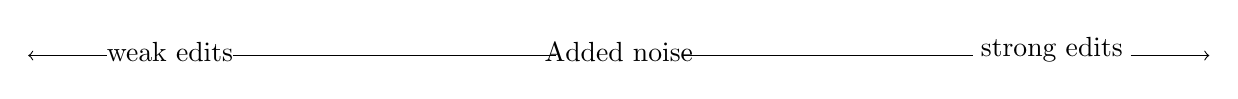
\begin{tikzpicture}
                \draw[<-] (0,0) -- (1,0);
                \draw[-] (2.6,0) -- (6.7,0);
                \draw[-] (8.3,0) -- (12,0);
                \draw[->] (14,0) -- (15,0);
                \node[above] at (1.8,-0.2) {weak edits};
                \node[above] at (7.5,-0.2) {Added noise};
                \node[above] at (13,-0.2) {strong edits};
            \end{tikzpicture}
        }\\[-4pt]%
        && 0.0 & 0.2 & 0.4 & 0.6 & 0.8 & \textbf{1.0}\\%
        \rotatebox{90}{\hspace*{4em}View 1}&%
        \includegraphics[height=0.14\linewidth]{figures/secondary_hparams/initial/0001.png}&%
        \includegraphics[height=0.14\linewidth]{figures/secondary_hparams/initial/0001.png}&%
        \includegraphics[height=0.14\linewidth]{figures/secondary_hparams/strength_0.2_001.jpg}&%
        \includegraphics[height=0.14\linewidth]{figures/secondary_hparams/strength_0.4_001.jpg}&%
        \includegraphics[height=0.14\linewidth]{figures/secondary_hparams/strength_0.6_001.jpg}&%
        \includegraphics[height=0.14\linewidth]{figures/secondary_hparams/strength_0.8_001.jpg}&%
        \includegraphics[height=0.14\linewidth]{figures/secondary_hparams/strength_1.0_001.jpg}\\%
        \rotatebox{90}{\hspace*{4em}View 2}&
        \includegraphics[height=0.14\linewidth]{figures/secondary_hparams/initial/0006.png}&%
        \includegraphics[height=0.14\linewidth]{figures/secondary_hparams/initial/0006.png}&%
        \includegraphics[height=0.14\linewidth]{figures/secondary_hparams/strength_0.2_006.jpg}&%
        \includegraphics[height=0.14\linewidth]{figures/secondary_hparams/strength_0.4_006.jpg}&%
        \includegraphics[height=0.14\linewidth]{figures/secondary_hparams/strength_0.6_006.jpg}&%
        \includegraphics[height=0.14\linewidth]{figures/secondary_hparams/strength_0.8_006.jpg}&%
        \includegraphics[height=0.14\linewidth]{figures/secondary_hparams/strength_1.0_006.jpg}\\%
    \end{tabular}%

    \caption{Expanded version of Figure~\ref{fig:hparams_usercontrol} from the main paper. Apart from the \emph{classifier-free guidance} parameter (top), the underlying diffusion models of our system expose two further parameters that can be tweaked by users. Both the strength at which the \emph{ControlNet tile} (middle) and the \emph{input noise} (bottom) are applied allow tweaking how much the generated material details will deviate from the base material. Numbers highlighted in bold indicate parameter ranges we use throughout the results in the paper.}
    \label{fig:hparams_usercontrol_suppl}
\end{figure*}
